\documentclass[a4paper,
amsfonts,
amssymb,
amsmath,
reprint,
showkeys,
nofootinbib,
twoside]{revtex4-2}
\usepackage[english]{babel}
\usepackage[utf8]{inputenc}
\usepackage[pdftex, pdftitle={Article}, pdfauthor={Author}, hidelinks]{hyperref} % For hyperlinks in the PDF
\hypersetup{
    colorlinks=true,
    linkcolor=blue,
    filecolor=magenta,
    urlcolor=cyan,
}
\usepackage{xcolor}
\usepackage{bm}
\usepackage{physics}
\usepackage{graphicx}
\DeclareMathAlphabet{\mymathbb}{U}{BOONDOX-ds}{m}{n} % Fancy E for Exp value
%\setlength{\marginparwidth}{2.5cm}


\bibliographystyle{apsrev4-1}

\begin{document}
\title{Comparing methods for regression and classification}

\author{Halvor Melkild}
    \email[Correspondence email address: ]{halvor.melkild@fys.uio.no}
    \affiliation{Department of Physics, University of Oslo}

\author{Martin Tømterud}
    \email[Correspondence email address: ]{martin.tomterud@uib.no}
    \affiliation{Department of Physics and Technology, University of Bergen}
    \affiliation{Centre for Materials Science and Nanotechnology, University of Oslo}

\author{\textcolor{blue}{\href{https://github.com/martintomterud/DA-ML}{Code available at git rep https://github.com/martintomterud/DA-ML}}}

\date{\today}

\begin{abstract}
Classification techniques in machine learning are a powerful set of tools with seemingly endless possible application. Here we study two methods of classification; feedforward neural networks and logistic regression. We apply the techniques to a study of breast cancer patients to predict which of the patients have developed cancer and which have not. Our findings indicate that for the simple datasets we are investigating, simple gradient descent methods perform as good as the ones that tune the learning rate. Furthermore, we obtain an accuracy score of 0.96 for large parts of the parameter space using logistic regression, and an accuracy score of 0.98 using the neural network.
\end{abstract}

\keywords{machine learning, stochastic gradient descent, neural networks, logistic regression}

\maketitle

\section{Introduction}

Classification is one of the fundamental problems in machine learning and it pertains to identify which predefined class a series of observations can be identified as. Applications of classification methods are endless in modern data science. They are common in diagnostics, where models trained on observations by doctors can help classify, for instance, what illness a patient has, or if they have a high risk of developing cancer. In physics it has become popular to use machine learning techniques in combination with density functional theory, for instance, to predict which atomic structure in a material that gives the smallest energy. Another common application is using classification to let computers read hand written text.

In the present work, we will apply classification to a set of breast cancer data in an attempt to classify whether or not a patient has developed malignant breast cancer. In doing so we will use two of the most common classification methods; logistic regression and neural networks.

Logistic regression is a more rigid method, that models the probability of an observation to lead to a given outcome. Neural networks are more adaptable and commonly used throughout data science. The method is very flexible and can be scaled to handle extremely complex problems, but also applied to simple binary classification problems, as we do here.

Regression methods are rooted in minimisation problems, and we therefore start our study by examining different minimisation techniques that all iterate on gradient descent. We progress by testing the implementation of our neural network with linear regression methods. Both these minimisation methods are tested on data generated by the Franke function. Finally, we compare and discuss the performance of the neural network and our implementation of logistic regression on the breast cancer data.

\section{Theory and Methods}

\subsection{Logistic Regression}

Logistic regression models the probability that a set of data features, or input variables, $\bm{x}^{(i)} = \{1, x_1, ... ,x_p\}$ leads to a certain response, $y_i$. We organise these observations in a  dataset $G = \{\mathbf{x}^{(i)}, y_i\}_{i = 1}^n$. In logistic regression the response is called a class, and the index $k$ indicates which class the outcome belongs to, where $k$ can take on the values $k = 1, 2, ... , K$, with $K$ being the total number of classes. The simplest case is $K = 2$, with $y_i \in [0, 1]$, and the probability given by the sigmoid function (also called the logistic function)
\begin{equation}
    \sigma(t) = \frac{1}{1 + e^{-t}}.
    \label{eq:sigmoid}
\end{equation}
The probability that the outcome $y_i$ belongs to the class 1 is therefore given by the logistic model,
\begin{equation}
    P(y_i = 1 \vert \bm{x}, \beta) = \frac{1}{1 + e^{-\beta \cdot \bm{x}}}.
\end{equation}
Similarly, the probability of $y_k$ belonging to the class 0 is given by
\begin{equation}
     P(y_i = 0 \vert \bm{x}, \beta) = 1 - P(y_i = 1 \vert \bm{x}, \beta).
\end{equation}
We have used the standard probability notation; $P(y\vert x)$ is the probability of observing $y$ given $x$.
The regression coefficients of our model is given by the vector $\beta = (\beta_0, \beta_1, ..., \beta_p)$. Our model is therefore similar to the standard linear regression models,
\begin{equation}
    \beta \cdot \bm{x} = \beta_0 + \sum_{i = 1}^p \beta_i x_i.
\end{equation}
In order to train the model we need to define a cost function. The best candidate for logistic regression is minimising the cross entropy. To arrive at it we use the principle of maximum likelihood. We follow the derivation in \cite[page 120]{Hastie} throughout this section. The likelihood, $L$, of all possible outcomes in $G$ can be approximated by the product of the probability of all outcomes. In other words,
\begin{equation}
    L(\beta) = \prod_{i = 1}^n P_i^{y_i}(1 - P_i)^{1 - y_i},
\end{equation}
where we have used the notation
\begin{equation}
    P_i = P(y_i = 1 \vert \bm{x}, \beta).
\end{equation}
The optimal regression coefficients $\beta$ are therefore the ones that maximises the likelihood, $L$. In this case it is mathematically easier to work with the logarithm of the likelihood,
\begin{equation}
    l(\beta) = \log [L(\beta)],
\end{equation}
because the logarithm converts the products into summations. The fact that the logarithm is a strictly monotonic function assures that $L(\beta)$ and $l(\beta)$ have the same solutions for the maximisation problem. We can therefore define our cost function as the negative logarithm of the likelihood,
\begin{equation}
\begin{split}
    C(\beta) &= -l(\beta) \\
    &= -\sum_{i = 1}^n (y_i \log (P_i) + (1 - y_i)\log(1 - P_i)).
\end{split}
\label{eq:cost}
\end{equation}
This is known as the cross entropy.

We can also study the cost function with an additional regularisation parameter $\lambda$, similar as in ridge regression. This is done by adding an $L_2$-term to the cross entropy, giving
\begin{equation}
    C_{\lambda}(\beta) = -l(\beta) + \lambda \lVert \bm{\beta}\rVert^2,
    \label{eq:ridge}
\end{equation}
Minimising $C(\beta)$ is equivalent to computing the gradient and equating to zero.  Taking the gradient with respect to $\beta$ and writing out the result in matrix form, we obtain,
\begin{equation}
    \nabla_{\beta}C(\beta) = - \bm{X}^T(\bm{Y} - \bm{P})
\end{equation}
Here, $\bm{X}$ is the design matrix, with the vector $\bm{x}^{(i)}$ on row $i$, $\bm{y} = (y_1, ..., y_n)$, and $\bm{P} = (P_1, ..., P_n)$.
The minimisation equation, $\nabla_{\beta}C(\beta) = 0$ has no analytical solutions, and we will therefore apply gradient descent methods in order to find the optimal $\beta$ parameters.

\subsection{Gradient Descent}
Gradient descent methods are widely used in machine learning problems to find the minimum of the cost function. The minimisation equations rarely have analytical solutions, and numerical methods falling under the "gradient descent"-umbrella are often used to compute the minima. We will present some of them here.

We will consider a general dataset $X$, with some model function $f(z)$ depending on the variables $z$. As with the case for logistic regression, we have defined a cost function $C(X, f)$. We will fit our model by finding the parameters $z$ that minimise $C$.

The standard form of gradient descent is called steepest descent. The derivation follows the lecture notes~\footnote{\href{https://compphysics.github.io/MachineLearning/doc/pub/week39/html/week39.html}{Week 39}}. If we want to minimise the function $F(\bm{x})$ that evaluates the vector $\bm{x} = (x_1, ... , x_n)$, the function $F$ decreases the fastest in the direction of the negative gradient. Thus, if we want to find the $\bm{x}$ that minimises the $F$ iteratively, we employ the algorithm
\begin{equation}
    \bm{x}_{i+1} = \bm{x}_i - \gamma_{i}\nabla F(\bm{x}_i).
\end{equation}
Here, $\gamma_i > 0$ is called the learning rate. For $\gamma_i$ small enough we are guaranteed that $F(\bm{x}_{i+1}) \leq F(\bm{x}_{i})$. This naive, first version of gradient descent is simple to implement, but comes with significant disadvantages. Most prominently, the minimum found by gradient descent is not guaranteed to be a global minimum, the algorithm is heavily dependent on the learning rate, and a gradient is computationally expensive to compute. Therefore several improvements to the gradient descent algorithm have been developed that aims to tackle these issues. We will go through some of them here, including the stochastic gradient descent (SGD) method that introduces randomness, momentum accelerated methods, and methods that tune the learning rate.

\subsubsection{Stochastic Gradient Descent (SGD)}

The crucial observation of the SGD method is that, in many cases, including Eq.~\eqref{eq:cost}, the cost function $C(\beta)$ can be written as a sum over $n$ independent data points,
\begin{equation}
    C(\beta) = \sum_{i = 1}^n c_i(\bm{x}_i, \beta)
\end{equation}
The implication is therefore that the gradient also can be written as a sum of $n$ independent gradients.
\begin{equation}
    \nabla_{\beta} C(\beta) =  \sum_{i = 1}^n \nabla_{\beta}c_i(\bm{x}_i, \beta)
\end{equation}

The randomness in the \textit{stochastic} gradient descent method is now introduces by dividing the $n$ independent datapoints into subsets, called minibatches. With $n$ datapoints and $M$ points in each minibatch, there are $n/M$ total minibatches. We denote the minibatch $B_k$, with $k \in [1, n/M]$. The total gradient is now approximated by only computing the gradient of one randomly chosen minibatch in each iteration step.

\begin{equation}
    \sum_{i = 1}^n \nabla_{\beta}c_i(\bm{x}_i, \beta) \approx \sum_{i \in B_k}^n \nabla_{\beta}c_i(\bm{x}_i, \beta)
\end{equation}

The minimisation step in SGD therefore reads

\begin{equation}
    \beta_{j+1} = \beta_j - \gamma_j  \sum_{i \in B_k}^n \nabla_{\beta}c_i(\bm{x}_i, \beta_j).
\end{equation}

The SGD method offers two major improvements to simple GD. Firstly, only computing the gradient of the randomly chosen minibatch in each step decreases computational cost, and cost reduction scales with system size. Secondly, randomly picking the minibatch in each step minimises the chance of getting stuck in a local minimum.

\subsubsection{Momentum accelerated methods}

One of the main drawbacks of the SGD method is that it has difficulties navigating in parameter space when the gradient is much steeper in one direction. This can lead to oscillations that are hard to combat using only SGD. The solution is to introduce a momentum term, which stores the gradient computed at the previous step. This accelerates the minimisation in the direction that is consistently decreasing, making rapid arbitrary oscillations less important. The minimisation step is updated to

\begin{equation}
    \beta_{j+1} = \beta_j - \eta \sum_{i \in B_k}^n \nabla_{\beta}c_i(\bm{x}_i, \beta_{j-1})  - \gamma_j  \sum_{i \in B_k}^n \nabla_{\beta}c_i(\bm{x}_i, \beta_j),
\end{equation}

where $\eta$ is the strength of the momentum term, usually with a value close to unity. We use a value of $\eta = 0.99$.

\subsubsection{Tuning the learning rate}

Momentum accelerated methods improves the SGD, but they can still do better. In particular, a lot of information is lost when we throw away the history of the computed gradients. We therefore introduce two methods that keep track of the moments of the gradients we compute; RMS prop and Adam. RMS prop keeps track of the second moment of the gradients, while Adam keeps track of both the second and the first moment.

For ease of notation, we denote the gradient at each iteration $t$ by
\begin{equation}
    g_t = \nabla_{\beta}C(\beta_t).
\end{equation}
In RMS prop, the second moment of the gradient is given by
\begin{equation}
    s_t = \mymathbb{E}[g_t^2].
\end{equation}
As we want to keep track of past gradients as well, we use a running average of the second moments given by
\begin{equation}
    s_{t} = \alpha s_{t - 1} + (1- \alpha)g_t^2.
\end{equation}
The coefficient $\alpha$ controls the averaging time of the second moment. Typically, the value is about $\alpha = 0.9$. The minimisation step is given by
\begin{equation}
    \beta_{t+1} = \beta_t -  \frac{\gamma_t}{\sqrt{s_t + \epsilon}} g_t.
\end{equation}
The coefficient $\gamma_t$ is as before the learning rate, and $\epsilon$ is a small constant introduced to prevent divergences. Typical values are of the order of $\epsilon \sim 10^{-8}$. As is evident from the equation above RMS prop effectively tunes the learning rate by virtue of the second moment. In directions where the norm of the gradient is large, the learning rate is reduced, and this speeds up convergence by allowing for the use of large learning rates in flat directions.

ADAM is an evolution of RMS prop that includes both the second and first moment. As above, we denote the gradient by $g_t$. The first moment is the defined as
\begin{equation}
    m_t =\mymathbb{E}[g_t].
\end{equation}
Introducing the parameters $\alpha_1$ and $\alpha_2$ to control the running averages of the first and second moments respectively, we compute them as
\begin{equation}
    m_{t} = \alpha_1 m_{t - 1} + (1- \alpha_1)g_t,
\end{equation}
and
\begin{equation}
    s_{t} = \alpha_2 s_{t - 1} + (1- \alpha_2)g_t^2.
\end{equation}
At the first iteration, both $m_0$ and $s_0$ are set equal to zero. This implies that the estimates are biased towards zero. This is counteracted by using bias-corrected estimates in the minimisation step. The bias-corrected first and second moments are given by
\begin{equation}
    \hat{m}_t = \frac{m_t}{1 - \alpha_1^t},
\end{equation}
and
\begin{equation}
    \hat{s}_t = \frac{s_t}{1 - \alpha_2^t}.
\end{equation}
Finally, the minimization step in the Adam algorithm reads
\begin{equation}
    \beta_{t+1} =  \beta_t - \gamma_t \frac{\hat{m}_t}{\sqrt{\hat{s}_t} + \epsilon},
\end{equation}
where again $\epsilon$ is a regularisation parameter and $\gamma_t$ is the learning rate.

\subsection{Error Metrics}

In order to compare our results between different methods we will use two different error metrics; the mean squared error (MSE) and the accuracy score.
The mean squared error between a prediction, $\mathbf{\tilde{y}}$, and the actual value, $\mathbf{y}$, is given by
\begin{equation}
    \textrm{MSE}(\bm{y}, \bm{\tilde{y}}) = \frac{1}{n}\sum_{i = 1}^n (y_i - \tilde{y}_i)^2.
\end{equation}
We will apply MSE to the minimisation problems when we test the gradient descent methods and the neural network.
Meanwhile, the accuracy score will be applied when we test the classification schemes. The score measures the percentage of correctly classified labels. For instance, a score of $0.8$ implies that 80\% of the data was correctly labelled. The score is therefore given by
\begin{equation}
    \textrm{accuracy} = \frac{1}{n}\sum_{i = 1}^n \delta(\tilde{y}_i - y_i),
\end{equation}
where the $\delta$-function returns 1 if the prediction is correctly labelled, and 0 otherwise.




\subsection{Neural Networks}

Artificial neural networks (ANN) is a class of algorithms where a collection of nodes, commonly referred to as neurons, are connected by graphs. Neural networks are inspired by how brains function. There are many different versions of ANNs, and herein we will focus on (one of) the most common implementations, namely multilayer perceptrons (MLP). The algorithm will feed the input data to the first layer of neurons, before it is propagated through the layers by the graphs connecting them. We employ the feedforward algorithm, implying that information only flows one way through the neuron network.

\subsubsection{Propagation}

The propagation of the information, $\mathbf{p}$, is controlled by a set of weights, $\mathbf{w}$, which determines the strength of the connection between the neurons. This is done in three steps, which are:
\begin{itemize}
    \item The input information $\mathbf{p}$, which is either the initial information or the output from the previous layer, is scaled with the strength of the connection,
    \begin{equation}
        \mathbf{p} \longrightarrow \sum_i^n w_i p_i.
    \end{equation}

    \item The bias of the neuron is added to the weighted input:
    \begin{equation}
        \sum_i^n w_i p_i \longrightarrow \sum_i^n w_i p_i + b.
    \end{equation}
    \item The computed argument is processed by the activation function, $f$, of the neuron to compute the output,
    \begin{equation}
        \tilde{\mathbf{p}} = f \left( \sum_i^n w_i p_i + b \right).
    \end{equation}
    \item The output is the input of the next layer.
\end{itemize}

Summarised the algorithm can be written out in one equation,
\begin{equation}
    \mathbf{p} \longrightarrow f(\mathbf{w}^T \mathbf{p} + b) = \tilde{\mathbf{p}}.
\end{equation}

\subsubsection{Activation functions}

There are multiple choices for activation functions in the feed forward neural network, and the choice of activation function partly determines the networks behaviour. For instance in our application to regression and classification problems, different activation functions will be chosen for the output layer of the model. Activation functions are needed to introduce non-linearity in the network, as without them the neural network would simply be a series of linear transformations.

For regression problems there are multiple possible options. We will apply the sigmoid function, introduced in Eq.~\eqref{eq:sigmoid}, the rectified linear unit function (ReLU) and the leaky ReLU functions. The last two are given by
\begin{equation}
    \textrm{ReLU}(t) =
    \begin{cases}
        0 \: &\textrm{ for } t < 0 \\
        t \: &\textrm{ for } t \geq 0
    \end{cases}
\end{equation}
and
\begin{equation}
    \textrm{Leaky ReLU}(t) =
    \begin{cases}
        0.01t \: &\textrm{ for } t < 0 \\
        t \: &\textrm{ for } t \geq 0
    \end{cases},
\end{equation}
respectively. As the output of the last layer in a regression model could be any real number, it does not make sense to add an activation function to this layer.

For the classification problem we will use the sigmoid function. This choice is suitable for binary classification, where the output is labelled to either 0 or 1. For the output layer we will simply round the output from the sigmoid to either 0 or 1. For multiclass classification the generalised choice would be the softmax function.

\subsubsection{Output and back propagation}
After the completion of the feed forward process, the output of the neural network is compared to the true values of the training data. The comparison is computed using the MSE in regression problems and the accuracy score in classification problems. Afterwards the weights and bias is adjusted and the process is repeated. One run of the feed forward algorithm is referred to as an epoch, while the adjustment of weights and biases is referred to as back propagation.

Comparing the output with the real values of the training data requires a cost function. The cost functions used for the neural network are the same as the ones we have already discussed. We will use the OLS and Ridge functions, studied in Project 1, in regression problems, and the cross entropy in Eq.~\eqref{eq:cost} for the classification problems.
The objective of the comparison is minimising the cost function, $C$. We employ gradient descent methods to do this, calculating the gradient of the cost function and updating the weights and bias in the direction of steepest descent, essentially applying the gradient descent methods already introduced. If we define the argument of the activation function, $f$, as
\begin{equation}
    t \equiv \mathbf{w}^T \mathbf{p} + b,
\end{equation}
then the gradient of the cost function of the output layer, $L$, is given by
\begin{equation}
    \epsilon_L = \frac{\partial C}{\partial f} \frac{\partial f}{\partial t_L}.
\end{equation}
We can then back propagate this error to the other layers $l = L- 1, L-2, ... , 2$ via
\begin{equation}
    \epsilon_l = \epsilon_{l+1} \mathbf{w}^T_{l+1} \frac{\partial f}{\partial t_l}
\end{equation}
The new weights and biases are thereafter calculated as \begin{equation}
    \mathbf{w}_l = \mathbf{w}_l - \gamma \epsilon_l \frac{\partial f}{\partial t_{l-1}},
\end{equation}
\begin{equation}
    b_l = b_l - \gamma \epsilon_l,
\end{equation}
where $\gamma$ is the learning rate.

\subsubsection{Initialisation of weights and bias}

The feedforward neural network is an iterative process and its general nature means that there is no guarantee for it to converge to a global minima, or even converge at all within the limits on computational time. Picking suitable initial conditions is therefore important for the performance of the model. Unfortunately, how to choose good initial conditions has been a poorly understood problem\cite{gbc16}.

One known important aspect is that every node should be initialised differently. As the feedforward network is fully connected, two equal nodes will simply stay equal through training and the complexity of the model will be reduced. The simplest way to avoid this is to initialise all nodes randomly, as the chance of getting many equal nodes is negligible.

It has been pointed out that the variance of the input and output from a layer should be approximately equal\cite{gb10}. In the case where the variance increases through the network, many of the nodes will be saturated (with a activation function like the sigmoid), meaning that the gradient is nearly vanishing. As a result the learning process slows down. In the other case, when the variance dies out, many of the nodes becomes similar and the complexity of the model decreases.

In our analysis we have tested different random distributions to see how the choice affects our network.

\subsection{Data Preparation}

Before we analyse our implementation of the neural network we want to gain an understanding of the various parameters at play. This we do by analysing various gradient descent methods on the Franke function. The Franke function is modelled on a $1000 \times 1000$ grid of random points spanning $x, y \in [0, 1]$.  We use $p = 5$ degree polynomials in our model and seek to find the best fit of the Franke function using gradient descent methods. We use the mean squared error (MSE) as the metric to compare the different methods. We learned from work on project 1 that ordinary least squares (OLS) regression worked well on the Franke data and we therefore compare our analysis to the MSE obtained using OLS regression. We employ scikit-learn's own implementation\footnote{\href{https://scikit-learn.org/stable/modules/generated/sklearn.linear_model.LinearRegression.html}{Scikit-learn linear regression.}} to compute the OLS result. All data was scaled using scikit-learn's standard scaler~\footnote{\href{https://scikit-learn.org/stable/modules/generated/sklearn.preprocessing.StandardScaler.html}{Standard Scaler}} before regression and classification. We split our data into a train/test ratio of 80/20.

\section{Results and Discussion}
\label{results}



\subsection{Gradient Descent Methods}
Figures \ref{fig:sgd_1} and \ref{fig:sgd_2} show results for the SGD and SGDM methods, for two different minibatch sizes (64 and 128, respectively). Both methods use the learning rates presented in the legend in the left panel of the figures.

\begin{figure} [h]
    \centering
    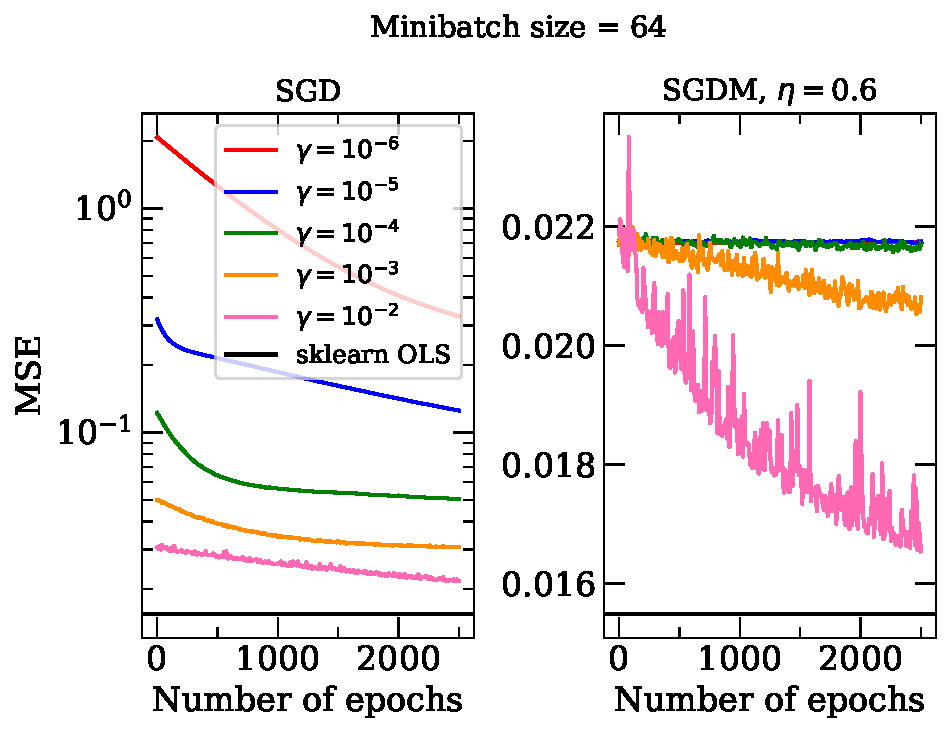
\includegraphics[width = \columnwidth]{Figures/sgd_1.pdf}
    \caption{Comparison of the MSE as a function of the number of epochs for the SGD and SGDM methods, using momentum $\eta = 0.6$ for the latter. The various learning rates are indicated in the legend in the left panel, and compared with the OLS result obtained using library methods shown as a horizontal black line. The minibatch size is indicated in the chart title. Note that the y axis is in logarithmic scale in the left panel. }
    \label{fig:sgd_1}
\end{figure}
\begin{figure} [h]
    \centering
    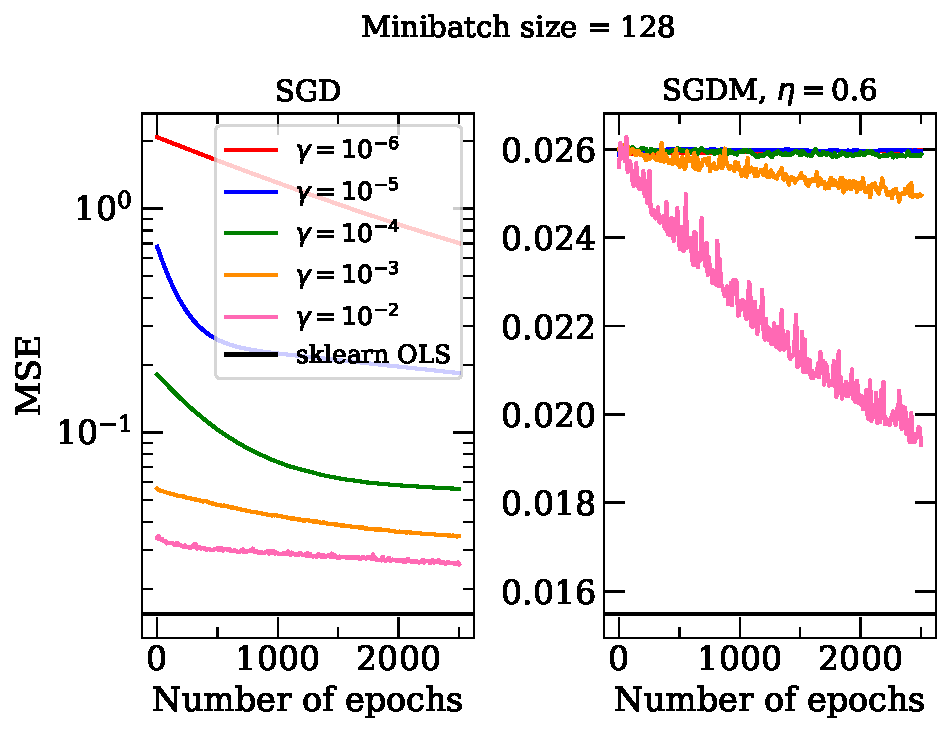
\includegraphics[width = \columnwidth]{Figures/sgd_2.pdf}
    \caption{Comparison of the MSE as a function of the number of epochs for the SGD and SGDM methods, using momentum $\eta = 0.6$ for the latter. The various learning rates are indicated in the legend in the left panel, and compared with the OLS result obtained using library methods shown as a horizontal black line. The minibatch size is indicated in the chart title. Note that the y axis is in logarithmic scale in the left panel.}
    \label{fig:sgd_2}
\end{figure}

Immediately, several interesting effects are observed. Firstly, for all instances the general observation is that the MSE approaches the OLS result, while the learning rate approaches unity. In other words, increasing the learning rate gives a faster convergence. Secondly, the inclusion of momentum gives a better MSE at smaller learning rates, but does not improve the MSE at the high learning rates that give a good MSE without momentum. However, the inclusion of momentum also implies a faster convergence for all learning rates. Thirdly, as the learning rate increases, we observe rapid oscillations in the MSE. Finally, of the two minibatch sizes tested, the smaller minibatch size gives the smallest MSE, but the advantage is minor.

Figure \ref{fig:sgd_ridge} shows SGD on the Franke function of where we have included an $L^2$ cost term in the cost function. The two panels in the Figure show the two learning rates that gave the smallest MSE in the previous example. We once again obtain the smallest MSE for the largest learning rate, but it does not outperform the MSE we found using the simple OLS cost function the previous figures. We also observe an interesting effect in the parameter $\lambda$ where the MSE initially decreases as $\lambda$ increases, but starts increasing again when $\lambda$ becomes too large. This is true for both learning rates.

\begin{figure} [h]
    \centering
    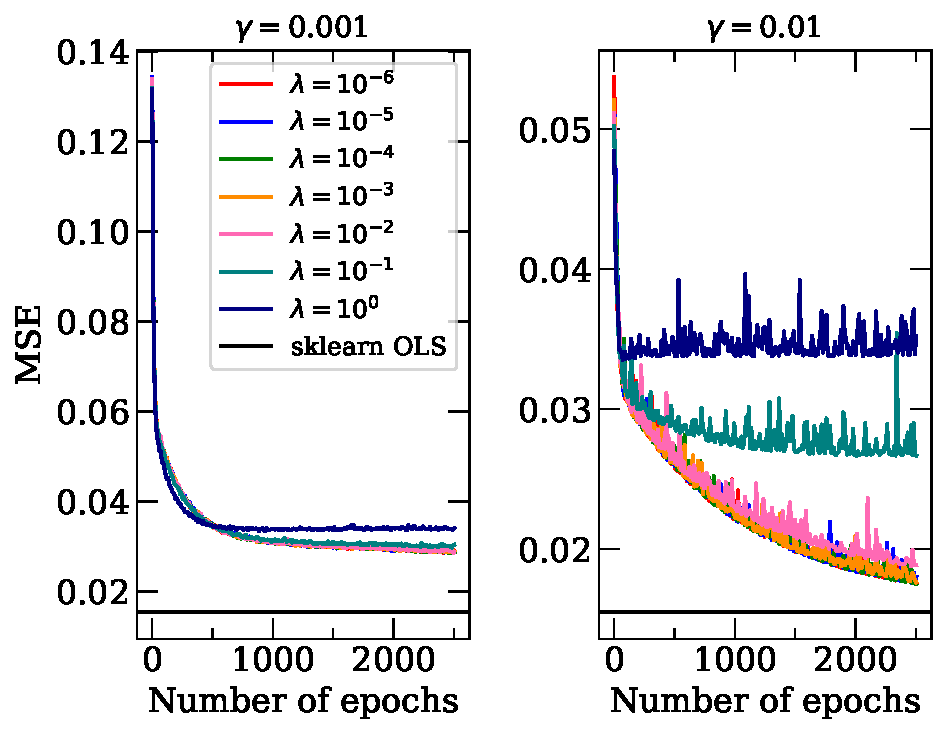
\includegraphics[width = \columnwidth]{Figures/sgd_ridge_1.pdf}
    \caption{The two learning rates that performed best for SGD investigated using an L2 penalty parameter $\lambda$, as indicated in the legend in the left panel. The results are compared with the OLS result obtained with library methods. }
    \label{fig:sgd_ridge}
\end{figure}



Figure \ref{fig:adagrad} investigates the adaptive gradient (adagrad) method with and without momentum. Again we observe that adding momentum yields a faster convergence, and here we observe that it also yields a slightly lower MSE for the larger learning rates.


\begin{figure}
    \centering
    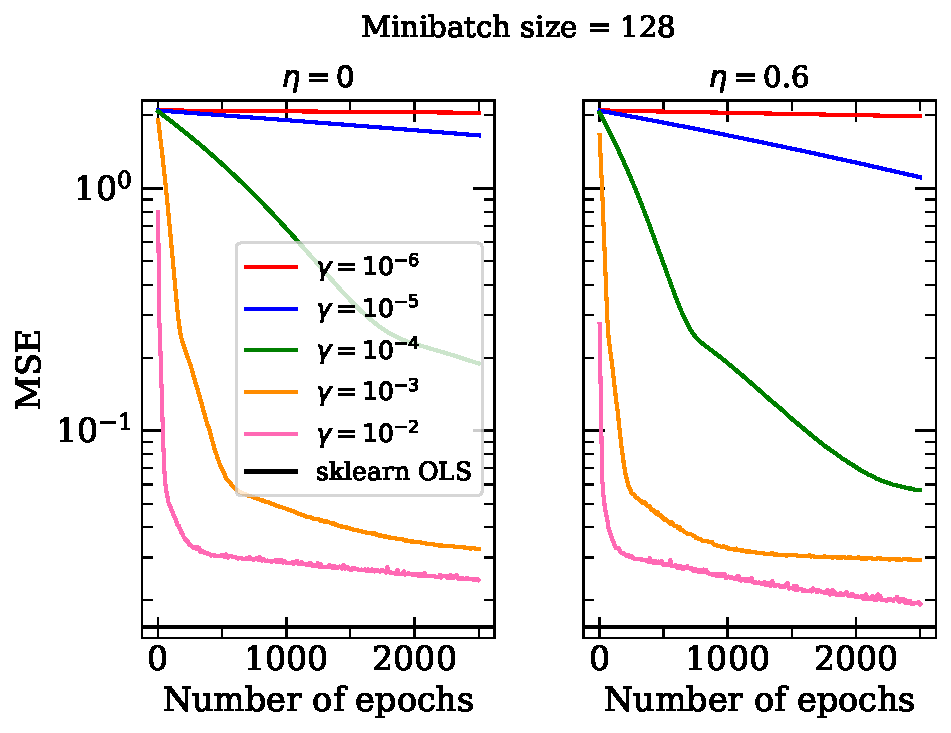
\includegraphics[width = \columnwidth]{Figures/adagrad_1.pdf}
    \caption{The adaptive gradient, or adagrad, method tested for various learning rates as indicated in the left panel legend and compared to the OLS result. The left panel shows the adagrad method tested without momentum, while the right panel shows the result using momentum $\eta = 0.6$.}
    \label{fig:adagrad}
\end{figure}

Finally, Figure \ref{fig:tunerates} compares two methods for tuning the learning rates, RMSprop and ADAM. These methods give the smallest MSE we observe, but they also feature the most rapid oscillations with the largest amplitudes.

\begin{figure}
    \centering
    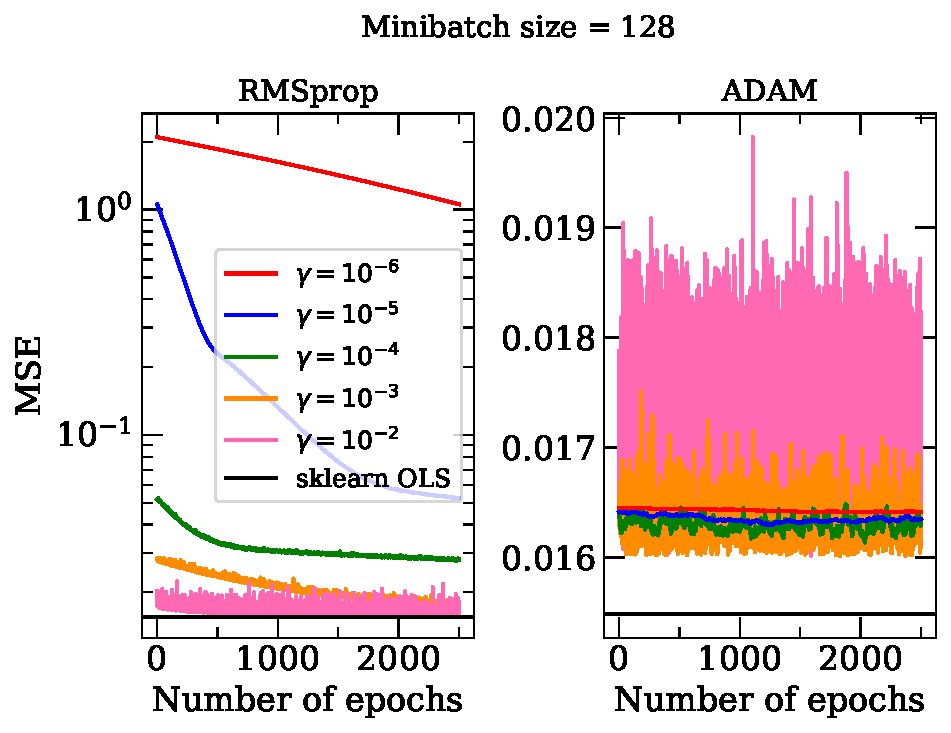
\includegraphics[width = \columnwidth]{Figures/tunerates_1.pdf}
    \caption{Comparison of the two SGD methods that tune the learning rate; RMSprop (left) and ADAM (right). The learning rates for both panles are indicated in the legend on the left side. The methods are compared to the OLS regression result. Note that the y-axis has log scale in the left panel.}
    \label{fig:tunerates}
\end{figure}

In all the methods we have investigated we find that when gradient descent method has converged it starts oscillating rapidly about a minimum. Intuitively the reasoning is simple for the SGD and SGDM methods with a fixed learning rate. Once the method locates a minimum and converges to it, it is unable to get closer to said minimum due to the finite size of the learning rate. This is often explained with the metaphor of a ball with a fixed energy in a frictionless well; it is unable to settle at the bottom of the well due to its finite energy (corresponding to the learning rate) and the energy is not lost to friction. The ball will therefore oscillate around the bottom of the well indefinitely. This issue could however be addressed by tuning the learning rate, making it decrease as we approach the minimum. However, the same oscillatory behaviour is also observed with the two methods that tune the learning rate, namely RMSprop and ADAM. Curiously, for ADAM we obtain a good, non-oscillating MSE when we start out with smaller learning rates. The oscillations increase with increasing learning rates, signalling that we either are unable to combat the curvature with tuning the learning rate, or that learning rates are not decreased on a fast enough time scale.

Another curios behaviour we observe is shown in Figure \ref{fig:sgd_ridge}, where too large penalty parameters $\lambda$ are seen to increase the MSE. This can be understood from Eq.~\eqref{eq:ridge}, where we add a constant term to the cost function, that is the product of the squared norm of the regression weights and the penalty parameter $\lambda$. This prevents the norm of the regression weights becoming too large, but it will also act as a constant addition to the weights when they otherwise are well converged. The constant addition increases with the size of $\lambda$, explaining why, in Figure~\ref{fig:sgd_ridge}, the converged MSE increases with the size of $\lambda$.

Summarising the analysis on gradient descent methods, we obtain good results for all investigated methods. The more complex methods, \textit{i.e.} adagrad, RMSprop and ADAM all give good, and when good parameters are chosen, slightly better MSE than the standard SGD and SGDM methods. However, they are more computationally expensive, with minimal to no gain. There are a couple of likely explanations for this. Firstly, we are training our methods on a relatively small dataset, and secondly, we are using a fairly limited number of epochs. For larger datasets, and with epoch numbers orders of magnitude larger than the ones we are using, it is likely that we would observe better performance of the more complex models.

\subsection{Neural Network}

The neural network was analysed using a simple SGD, with constant learning late. Figure~\ref{fig:nn1} shown the development of the loss during training on the Franke function for different learning rates. As was the case for the linear model above, we see that for small learning rates, the convergence goes very slowly. The optimal value lies in the interval $0.5-0.8$. When we increased the learning rate beyond $1$, the network becomes unstable.

Similar to previously we got no improvement from including a regularisation parameter, $\lambda$, for the fit to the Franke function.

For the initial weights, we found that a normal distribution with a standard deviation of around 2, gave the best fit to the data. For a distribution with standard deviation less than 0.1, we found that the training never got going. For higher standard deviation the network became unstable.

Having fixed the parameters discussed above we adjusted the number of nodes per layer and number of layers. Starting with a single layer, the performance improved from going from 1 to around 20 layers. Further, it stabilised until we reached about 90 layers, when the model started overfitting.

\begin{figure}
    \centering
    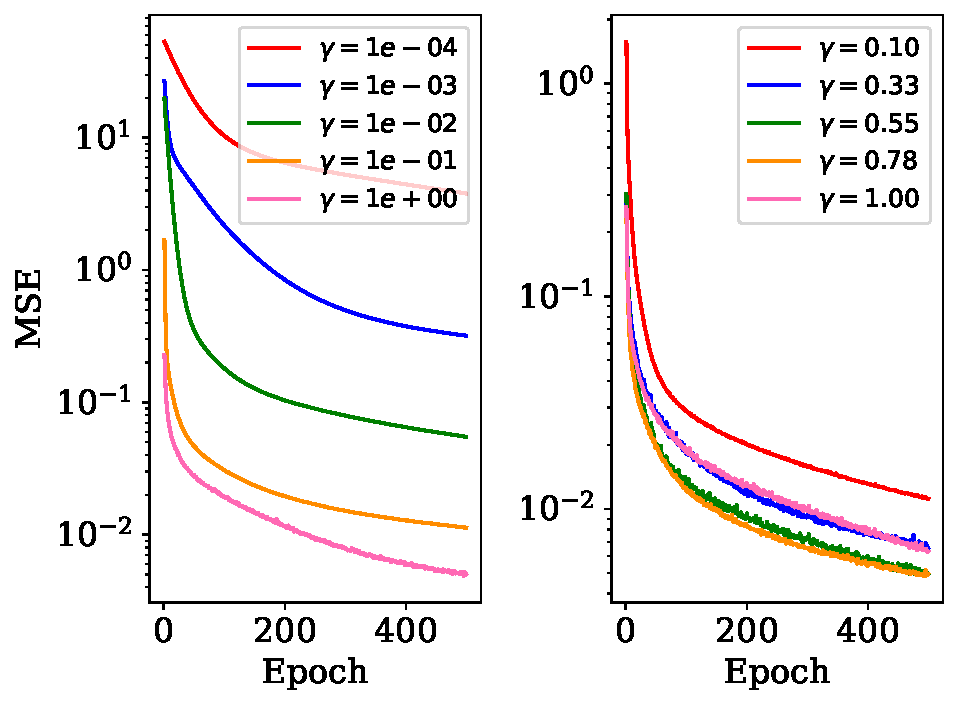
\includegraphics[width = \columnwidth]{Figures/lr_test.pdf}
    \caption{Feedforward neural network tested for various learning rates. We see that the fit converges faster for higher learning rates, up to order 1.}
    \label{fig:nn1}
\end{figure}

Having tested the network on the Franke function we adopted it to the classification problem of the breast cancer data set. The only changes we did was changing the cost function to the cross entropy and using adding the sigmoid function also to the output layer. In Figure~\ref{fig:nn3} we present the accuracy scores for a set of learning rates and regularisation parameters. Again we see that the performance does not depend heavily on the regularisation parameter. We see that the network performs very well with score around 0.97 at the learning rate 0.1.

\begin{figure}
    \centering
    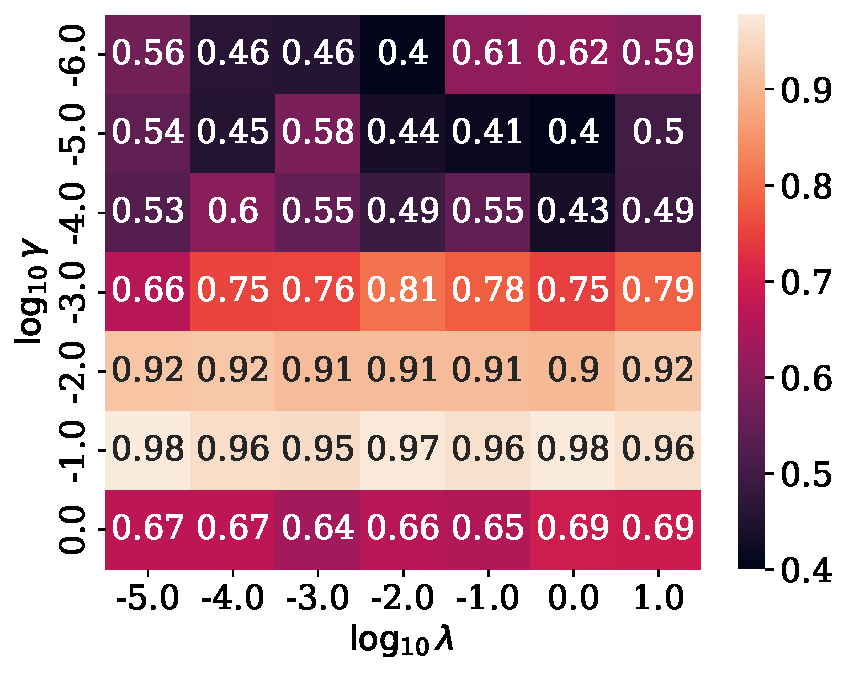
\includegraphics[width = \columnwidth]{Figures/logreg.pdf}
    \caption{Accuracy matrix for the feedforward neural classifier, tested on the breast cancer dataset. The network consists of a single layer with 50 nodes.}
    \label{fig:nn3}
\end{figure}

\subsection{Classification and Logistic Regression}

Accuracy score matrices for classification of breast cancer data using logistic regression are presented in Figures~\ref{fig:logreg1} and \ref{fig:logreg2}, the latter with a momentum term in the gradient descent minimisation. In both cases we obtain a good accuracy in a large portion of the explored parameter space, but with the momentum term yielding a better accuracy in the "worst" squares. This is in line with our observations from the initial comparison of the SGD/SGDM methods.

\begin{figure}
    \centering
    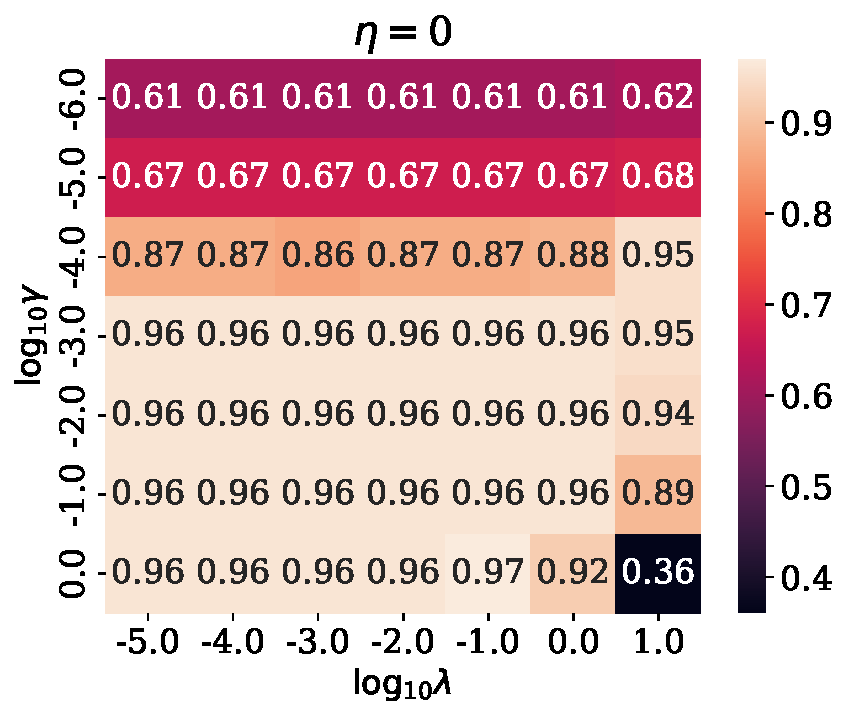
\includegraphics[width = \columnwidth]{Figures/logreg_no_mom.pdf}
    \caption{Accuracy matrix for logistic regression on the breast cancer dataset for various values of the learning rate, $\gamma$, and the regularisation parameter, $\lambda$, without momentum in the gradient descent method.}
    \label{fig:logreg1}
\end{figure}

\begin{figure}
    \centering
    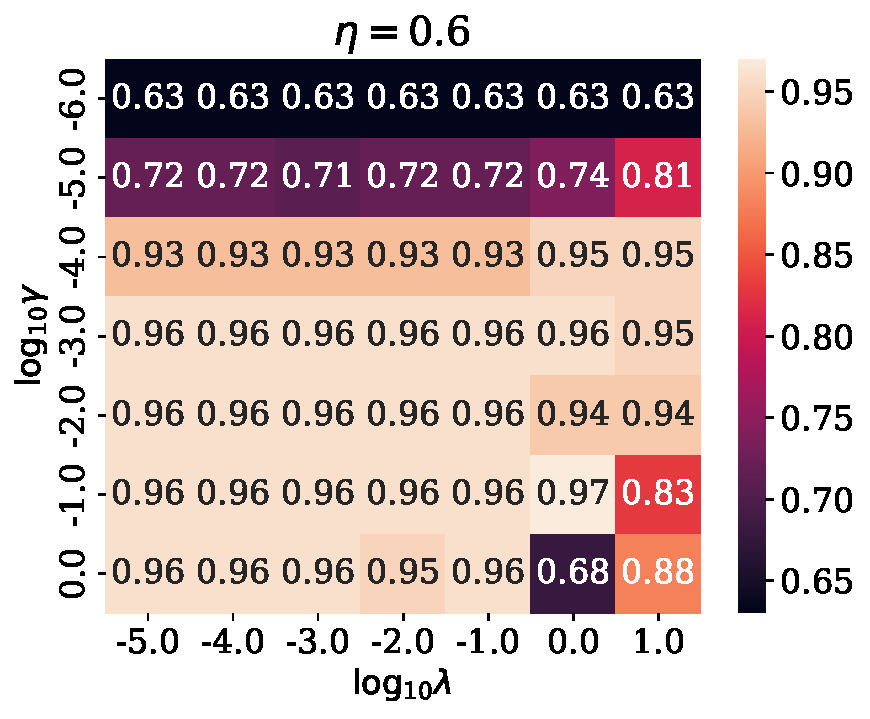
\includegraphics[width = \columnwidth]{Figures/logreg_mom.pdf}
    \caption{Accuracy matrix for logistic regression on the breast cancer dataset for various values of the learning rate, $\gamma$, and the regularisation parameter, $\lambda$, with momentum $\eta = 0.6$ in the gradient descent method.}
    \label{fig:logreg2}
\end{figure}

In both cases we also observe the same effect for the regularisation parameter $\lambda$ as we did when exploring it using SGD methods earlier. This holds true for large learning rates.
We also ran scikit-learn's implementation of logistic regression on the same dataset, obtaining an accuracy score of 0.99. Our implementation therefore performs well compared to the benchmark, albeit not perfect.


\section{Conclusion}

In this project we have compared gradient descent methods with neural networks applied to regression problems, and neural networks with logistic regression on classification problems.
For the regression problems we have extended the work of project 1 where OLS, Ridge and Lasso regression were applied to the Franke function. We find good convergence of all gradient descent methods applied, but find no real advantage of using computationally expensive adaptive methods on the "simple" problem we are dealing with in this project. As the standard SGD and SGDM methods achieve just as good MSE as the more advanced methods, these are the preferred choices when handling simple regression problems. Nevertheless, more advanced methods are likely to outperform them for more complex and large data sets.
The neural network also performs well for regression problems, achieving an MSE comparable to the standard deviation of the noise.

For the classification problem we have studied a breast cancer data set. The logistic regression method achieves an accuracy of 0.96 for a large portion of the parameter space, which is not too far from the benchmark accuracy of 0.99 obtained by the library method. The neural network is more dependent on the learning rate, but is able to score even better than logistic regression given the right learning rate.

%Bibliography
% \bibliographystyle{unsrt}
\bibliography{literature}

% \begin{thebibliography}{4}


% \bibitem{Hastie}
% T.~Hastie, R.~Tibshirani, and J.~Friedman.
% \textit{The Elements of Statistical Learning}.
% Springer, New York, 2009.

% \bibitem{Franke}
% R. Franke
% \textit{A Critical Comparison of Some Methods for Interpolation of Scattered Data}
% Naval Postgraduate School, California, 1979.

% \bibitem{James}
% G.~James, D.~Witten, T.~Hastie, and R.~Tibshirani.
% \textit{An Introduction to Statistical Learning}.
% Springer, New York, 2017.

% \bibitem{Hoerl}
% A.~E.~Hoerl, R.~W.~Rennard, (1970). Ridge Regression: Biased Estimation for Nonorthogonal Problems. \textit{Technometrics}, 12(1), 55–67.

% \end{thebibliography}


\end{document}
